\newpage % Rozdziały zaczynamy od nowej strony.

\section{Wyniki}
Poniższe dane przedstawione na rysunku \ref{fig:memories} prezentują ilość pamięci RAM wyrażonej w gigabajtach potrzebnej do uruchomienia poszczególnych architektur dla rozwiązania klasycznego oraz wykorzystującego wektor składający się z danych z map szczegółów sieci splotowych.
\begin{figure}[H]
    \centering
    \begin{subfigure}{.5\textwidth}
        \centering
        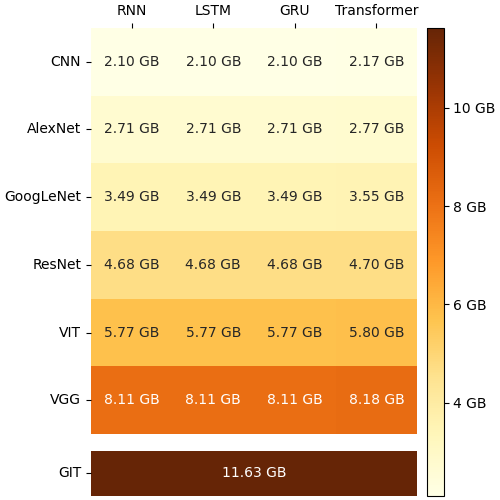
\includegraphics[width=.99\linewidth]{timings/ram}
        \caption{Klasyczne połączenie.}
        \label{fig:memory}
    \end{subfigure}%
    \centering
    \begin{subfigure}{.5\textwidth}
        \centering
        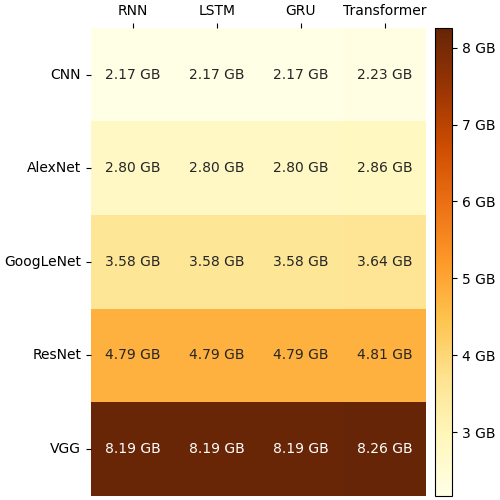
\includegraphics[width=.99\linewidth]{timings/ram_modified}
        \caption{Połączenie wykorzystujące mapy szczegółów.}
        \label{fig:memory-modified}
    \end{subfigure}%
    \caption{Pamięć RAM potrzebna do uruchomienia testowanych architektur wyrażona w gigabajtach. Opracowanie własne.}
    \label{fig:memories}
\end{figure}
\noindent Można zauważyć, iż największe różnice w ilości potrzebnej pamięci RAM są pomiędzy poszczególnymi modułami kodującymi. W przypadku modułów dekodujących zauważalna różnica jest pomiędzy wykorzystaniem transformera a pozostałymi sieciami rekurencyjnymi. Najpewniej wynika to z tego, iż sieci rekurencyjne przetwarzają tylko jeden element w danym czasie w przeciwieństwie do transformera, który przy pomocy modułu atencji analizuje całą sekwencję w jednym momencie, przez co konieczne jest jej załadowanie do pamięci komputera. Istotnym jest również fakt, iż połowa modułów kodujących potrzebuje ponad 4 GB pamięci, a co za tym idzie, nie było możliwe ich wykorzystanie przy pomocy karty graficznej Nvidia GeForce GTX 1650, ponieważ posiada ona tylko cztery gigabajty pamięci. Tak duża ilość potrzebnej pamięci dotyczy bardzo głębokich sieci oraz wykorzystujących transformer wizyjny. Powodem takiego stanu rzeczy jest fakt, iż w przypadku bardzo głębokich sieci splotowych architektura posiada ogromną liczbę parametrów ze względu na dużą liczbę małych filtrów oraz warstw. Natomiast transformer wizyjny przetwarza obraz do postaci sekwencji, która musi być załadowana w całości, co również znacząco wpływa na rozmiar potrzebnej pamięci. Warto również zauważyć, iż wykorzystanie danych pochodzących z map szczegółów sieci splotowych, tylko nieznacznie wpłynęło na zwiększenie wykorzystywanej pamięci RAM. Wpływ tutaj miało wykorzystanie warstw w pełni połączonych, które w porównaniu do warstw splotowych nie są aż tak obciążające i zajmują stosunkowo mniejszą ilość pamięci.

\subsection{Wydajność uczenia modułów dekodujących dla połączenia klasycznego}
Dane przedstawione na rysunku \ref{fig:timings-decoders} prezentują czas potrzebny na przetworzenie jednej epoki treningowej poszczególnych kombinacji modułów kodujących oraz dekodujących wykorzystujących wcześniej wytrenowane moduły kodujące przy pomocy klasycznego połączenia.
\begin{figure}[H]
    \centering
    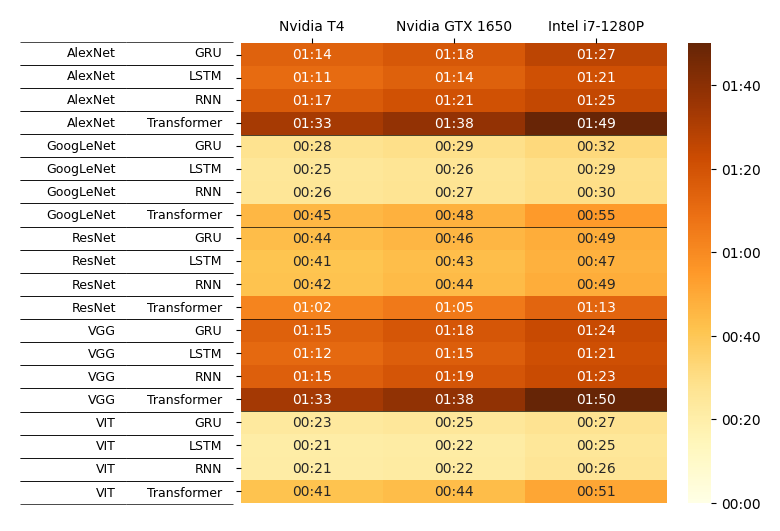
\includegraphics[width=.9\linewidth]{timings/timings_decoders}
    \caption{Czas potrzebny na przetworzenie jednej epoki treningowej poszczególnych kombinacji modułów kodujących oraz dekodujących wykorzystujących wcześniej wytrenowane moduły kodujące. Dane przedstawione w skali logarytmicznej. Opracowanie własne.}
    \label{fig:timings-decoders}
\end{figure}
\noindent Ponownie tak jak w przypadku potrzebnej pamięci do alokacji architektury tutaj również najbardziej zauważalne są różnice czasowe pomiędzy poszczególnymi modułami kodującymi. W przypadku modułów dekodujących różnice są widoczne jedynie pomiędzy wykorzystaniem transformera a pozostałymi sieciami rekurencyjnymi. Co ciekawe, długość przetwarzania nie jest zależna od stopnia skomplikowania sieci. Ze względu na wcześniejsze wygenerowanie danych wejściowych do modułów dekodujących poprzez przetworzenie obrazów przy pomocy wstępnie wyuczonych modułów kodujących, czas potrzebny na przetworzenie jednej epoki treningowej jest zależny od wielkości ostatniej warstwy modułu kodującego, który jest następujący dla poszczególnych sieci:
\begin{itemize}
    \item AlexNet -- 4096,
    \item GoogLeNet -- 1024,
    \item VGGNet -- 4096,
    \item ResNet -- 2048,
    \item VIT -- 768.
\end{itemize}
Biorąc to pod uwagę, łatwo można zauważyć, iż sieć z najmniejszą warstwą końcową, czyli VIT, potrzebuje najmniej czasu na przetworzenie jednej epoki treningowej, a sieci z największą warstwą końcową, czyli AlexNet oraz VGGNet, potrzebuje go najwięcej. W przypadku trenowania również modułu kodującego bez zastosowania wstępnie wyuczonych modeli możliwe byłoby dostosowanie wielkości ostatniej warstwy, w celu zmniejszenia czasu potrzebnego na przetworzenie danych przez moduł dekodujący.
\subsection{Wydajność uczenia architektury dla zaproponowanego połączenia}
W przypadku wykorzystania dodatkowych danych pochodzących z pośrednich warstw splotowych konieczne było zastosowanie warstw w pełni połączonych, które również musiały zostać wytrenowane wraz z modułem dekodującym. Dane przedstawione na rysunku \ref{fig:timings-decoders-modified} prezentują czas potrzebny na przetworzenie jednej epoki treningowej poszczególnych kombinacji modułów kodujących oraz dekodujących wykorzystujących wcześniej wytrenowane moduły kodujące przy pomocy zaproponowanego połączenia.
\begin{figure}[H]
    \centering
    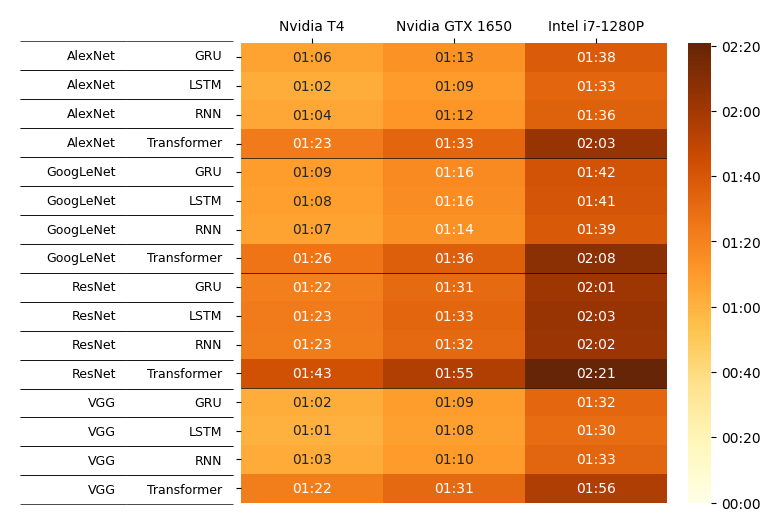
\includegraphics[width=.9\linewidth]{timings/timings_decoders_modified}
    \caption{Czas potrzebny na przetworzenie jednej epoki treningowej poszczególnych kombinacji modułów kodujących oraz dekodujących wykorzystujących wcześniej wytrenowane moduły kodujące przy pomocy zaproponowanego połączenia. Opracowanie własne.}
    \label{fig:timings-decoders-modified}
\end{figure}
\noindent Ze względu na generowanie wektorów wejściowych o takich samych rozmiarach dla każdego z modułów kodujących, różnica pomiędzy ich poszczególnymi typami nie jest tak widoczna, jak w przypadku klasycznego podejścia. W przypadku sieci AlexNet oraz VGG, których rozmiar wyjściowych wektorów pozostał niezmienny, wzrost czasu jest na poziomie około 10\%, co jest przewidywalną różnicą ze względu na konieczność wyuczenia również warstw w pełni połączonych odpowiedzialnych za redukcję rozmiaru wektorów pochodzących z warstw splotowych. Tak jak w poprzednim przypadku, ponownie można zauważyć różnicę pomiędzy sieciami rekurencyjnymi a transformerem. Również warto zwrócić uwagę na to, iż wykorzystanie jednostki GPU miało pewien wpływ na wydajność treningu, ale nie była to drastyczna poprawa -- w większości przypadków spadek czasu wyniósł około 25\% w przypadku podstawowej jednostki GPU, a około 30\% w przypadku jednostki specjalistycznej w porównaniu do jednostki CPU. Można stwierdzić, iż wykorzystanie danych z warstw splotowych miało wpływ na długość treningu, mimo iż jest to jedynie kilka sekund przetwarzania epoki, biorąc pod uwagę fakt, iż w przypadku trenowania sieci konieczne jest przetworzenie danych kilkaset razy, różnica ta staje się znacząca -- przetworzenie 250 epok daje różnicę na poziomie 45 minut.
\subsection{Wydajność uczenia modułów kodujących oraz dekodujących}
Dane przedstawione na rysunku \ref{fig:timings-networks} prezentują czas potrzebny na przetworzenie jednej epoki treningowej poszczególnych kombinacji modułów kodujących oraz dekodujących.
\begin{figure}[H]
    \centering
    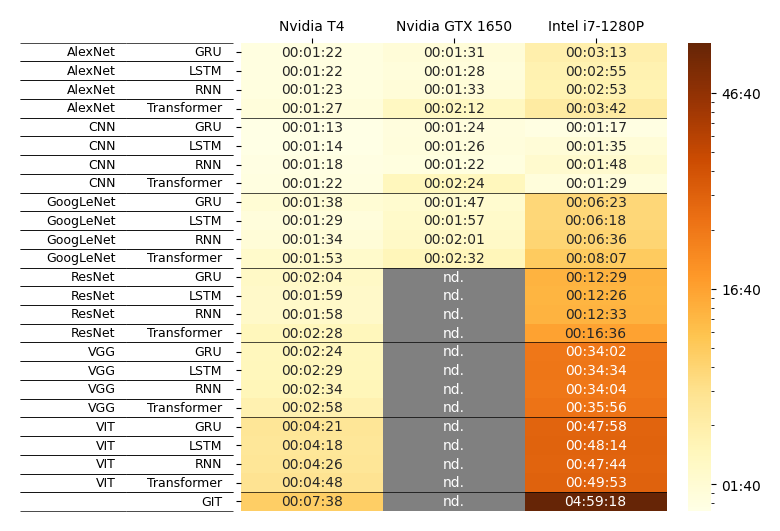
\includegraphics[width=.9\linewidth]{timings/timings_networks}
    \caption{Czas potrzebny na przetworzenie jednej epoki treningowej poszczególnych kombinacji modułów kodujących oraz dekodujących. Opracowanie własne.}
    \label{fig:timings-networks}
\end{figure}
\noindent Niestety ze względu na ograniczenie pamięci RAM karty graficznej Nvidia GTX 1650 nie było możliwe przeprowadzenie treningu sieci zajmujących więcej niż 4 GB pamięci, czyli ResNet, VGG, VIT oraz GIT. W przypadku czasu potrzebnego na przetworzenie danych przy pomocy jednostki CPU rośnie on w sposób wykładniczy. Biorąc pod uwagę, iż założeniem przeprowadzonych eksperymentów było przetworzenie zbioru treningowej 500 razy, dla połowy sieci staje się to niewykonalne. Już w przypadku sieci GoogleNet połączonej z jedną z sieci rekurencyjnych, gdzie jedna epoka treningowa zajmuje ponad 6 minut, powtórzenie jej 500 razy zajęłoby 53 godziny. Natomiast w przypadku najdłużej przetwarzającej sieci, czyli GIT, czas ten wyniósłby ponad 100 dni ciągłego przetwarzania. W przypadku pozostałych sieci, gdzie czas kilkudziesięciu godzin jest w wielu momentach akceptowalnym rzędem wielkości, to tak wydłużony czas uczenia znacząco utrudnia reagowanie na wszelkie błędy oraz problemy. Sytuacja jest znacznie lepsza w przypadku wykorzystania jednostki GPU. Pomiędzy modelem dostępnym w wielu komputerach stacjonarnych, Nvidia GTX 1650, a modelem dedykowanym do obliczeń na kartach graficznych, Nvidia T4, różnice są stosunkowo niewielkie. W przypadku architektury GIT przetworzenie danych 500 razy zajęłoby około 65 godzin, co w porównaniu do czasu potrzebnego w przypadku wykorzystania jednostki CPU jest osiągalne. Dodatkowo warto wspomnieć, iż korelacja pomiędzy liczbą parametrów ostatniej warstwy modułu kodującego a czasem potrzebny na trening nie pojawia się w tym przypadku. Wynika to z faktu, iż czas trenowania modułu kodującego rośnie o wiele znaczniej wraz z większym skomplikowaniem wykorzystanej architektury. Z tego względu również różnice pomiędzy architekturami wykorzystującymi klasyczne połączenie modułów a tymi wykorzystującymi dodatkowe dane z warstw splotowych nie są aż tak zauważalne -- wzrost czasu treningu jest nieznaczny w porównaniu do całościowego czasu przetwarzania, co można zauważyć na rysunku \ref{fig:timings-networks-modified}.
\begin{figure}[H]
    \centering
    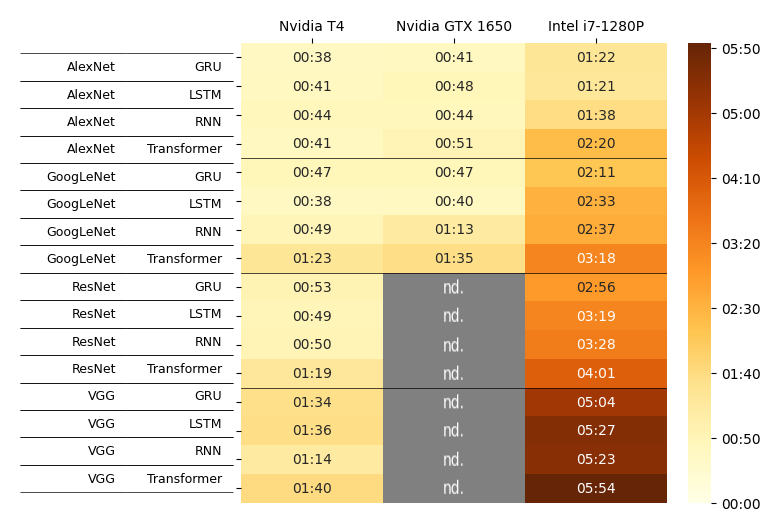
\includegraphics[width=.9\linewidth]{timings/timings_inference_decoders_modified}
    \caption{Czas potrzebny na przetworzenie jednej epoki treningowej poszczególnych kombinacji modułów kodujących oraz dekodujących wykorzystujących dane z warstw splotowych. Opracowanie własne.}
    \label{fig:timings-networks-modified}
\end{figure}
\noindent Różnica w czasie trenowania pomiędzy klasyczną techniką połączenia modułu kodującego i dekodującego a zaproponowanym rozwiązaniem wykorzystującym dane z warstw splotowych jest bardzo zbliżona w obu przypadkach -- trenowania modułu dekodującego oraz całej architektury. Jest to przewidywalny rezultat, ponieważ w obu podejściach dodatkowe obciążenie jest takie samo -- konieczność wyuczenia dodatkowych warstw w pełni połączonych.
\subsection{Wydajność generowania podpisów}
Na rysunku \ref{fig:timings-decoders-inference} zostały przedstawione czasy potrzebne na wygenerowanie podpisów obrazków pochodzących z testowego zbioru danych dla poszczególnych architektur.
\begin{figure}[H]
    \centering
    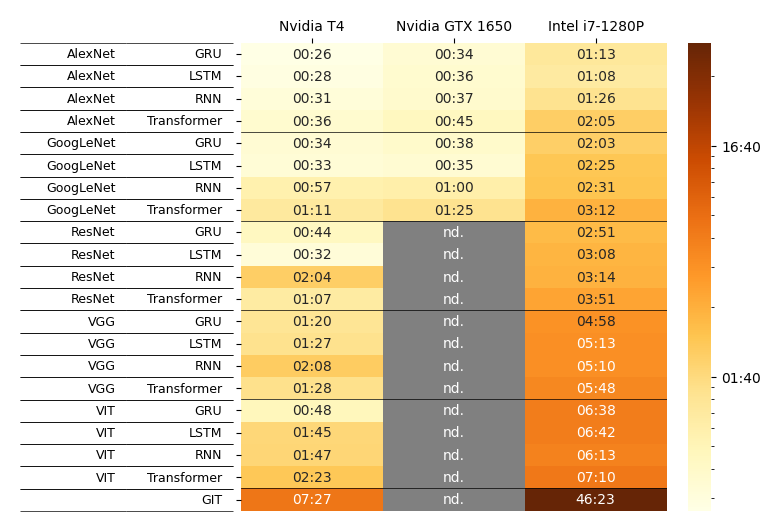
\includegraphics[width=.9\linewidth]{timings/timings_inference_decoders}
    \caption{Czas potrzebny na wygenerowanie podpisów obrazków pochodzących z testowego zbioru danych dla poszczególnych architektur, które zostały wyuczone przy użyciu wcześniej wytrenowanych modułów kodujących, wykorzystując klasyczne połączenie modułów. Dane przedstawione w skali logarytmicznej. Opracowanie własne.}
    \label{fig:timings-decoders-inference}
\end{figure}
\noindent W przypadku generowania podpisów konieczne jest wykorzystanie bezpośrednio modułu kodującego, ponieważ w warunkach naturalnych przetwarzane zdjęcie nie jest wcześniej znane. Z tego względu wyniki dla modeli wykorzystujących wcześniej wyuczone moduły kodujące oraz modele trenowane od zera są takie same -- w obu przypadkach obraz przetwarzany jest w ten sam sposób. Wskutek tego nie było możliwe przeprowadzenie eksperymentów przy użyciu karty graficznej Nvidia GTX 1650, tych sieci, których alokacja przekracza 4 GB pamięci. Czas wymagany do przetworzenia zbioru testowego, tak jak w przypadku uczenia architektur, wraz z wykorzystaniem bardziej rozbudowanego modułu kodującego wzrasta, a w przypadku modułów dekodujących znaczące różnice są widoczne jedynie pomiędzy transformerem a pozostałymi sieciami. Ponownie najbardziej wymagającą architekturą okazało się rozwiązanie GIT. Przy jego pomocy przetworzenie tysiąca zdjęć zajęłoby ponad 45 minut, co daje niecałe 3 sekundy na zdjęcie -- taki czas w wielu przypadkach można uznać za akceptowalny, jednakże ponownie pokazuje to, iż prostsze sieci są bardziej przystępne dla osób z ograniczonymi zasobami sprzętowymi. Najszybsza okazała się sieć AlexNet połączona z siecią GRU -- w tym przypadku przetworzenie całego zbioru testowego zajmuje mniej niż pół minuty.
W przypadku wykorzystania danych z wewnętrznych warstw splotowych modułu kodującego, w celu wygenerowania wektora wejściowego modułu kodującego czas generowania podpisów nie zmienił się znacząco, co można zauważyć na rysunku \ref{fig:timings-decoders-inference-modified}.
\begin{figure}[H]
    \centering
    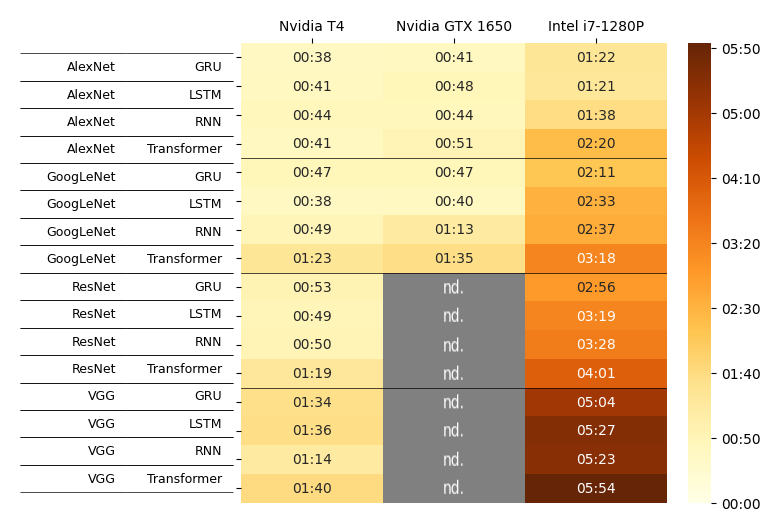
\includegraphics[width=.9\linewidth]{timings/timings_inference_decoders_modified}
    \caption{Czas potrzebny na wygenerowanie podpisów obrazków pochodzących z testowego zbioru danych dla poszczególnych architektur, które zostały wyuczone przy użyciu wcześniej wytrenowanych modułów kodujących, wykorzystując dane z warstw splotowych. Dane przedstawione w skali logarytmicznej. Opracowanie własne.}
    \label{fig:timings-decoders-inference-modified}
\end{figure}
\noindent Tak jak w pozostałych przypadkach, główna różnica czasowa pomiędzy klasycznym podejściem a wykorzystaniem warstw splotowych wynika z konieczności przetworzenia danych przy pomocy dodatkowych warstw w pełni połączonych. Wzrost czasu wynosi kilka sekund i nie jest to znacząco różnica, biorąc pod uwagę długość przetwarzania całego zbioru testowego.
\subsection{Skuteczność architektury wykorzystującej klasyczne połączenie}
Wydajność architektur jest niezwykle istotna, ale by móc w pełni ocenić ich przydatność, konieczne jest sprawdzenie skuteczności generowania podpisów. W tym celu wykorzystane zostały metryki BLEU oraz CIDEr. Dane przedstawione na rysunku \ref{fig:metrics} prezentują wartości tychże metryk dla architektury GIT oraz poszczególnych kombinacji modułów kodujących i dekodujących. Wyraźnie widoczna jest bardzo duża skuteczność architektury GIT. W przypadku metryki BLEU jest ona większa jedynie o 0,02 od drugiej najlepszej architektury -- kodera VIT połączonego z transformerem, ale w przypadku metryki CIDEr różnica ta jest już znacznie większa, ponieważ wynosi aż 0,16. Może to świadczyć o lepszej jakości generowanych podpisach. W przypadku wykorzystywania sieci RNN osiągnięcie sensownych wyników było niemożliwe.
\begin{figure}[H]
    \centering
    \begin{subfigure}{.5\textwidth}
        \centering
        \includegraphics[width=.95\linewidth]{metrics/BLEU}
        \caption{Wartości metryki BLEU}
        \label{fig:bleu}
    \end{subfigure}%
    \centering
    \begin{subfigure}{.5\textwidth}
        \centering
        \includegraphics[width=.95\linewidth]{metrics/CIDEr}
        \caption{Wartości metryki CIDEr}
        \label{fig:cider}
    \end{subfigure}%
    \caption{Wartości metryk BLEU oraz CIDEr dla poszczególnych kombinacji modułów kodujących i dekodujących. Opracowanie własne}
    \label{fig:metrics}
\end{figure}
\noindent W prawie wszystkich przypadkach funkcja straty zbioru walidacyjnego szybko osiągała swoje minimum, zaczynała rosnąć, co najczęściej sygnalizuje przeuczenie modelu -- można to zauważyć na rysunku \ref{fig:training-alexnet-rnn}.
\begin{figure}[H]
    \centering
    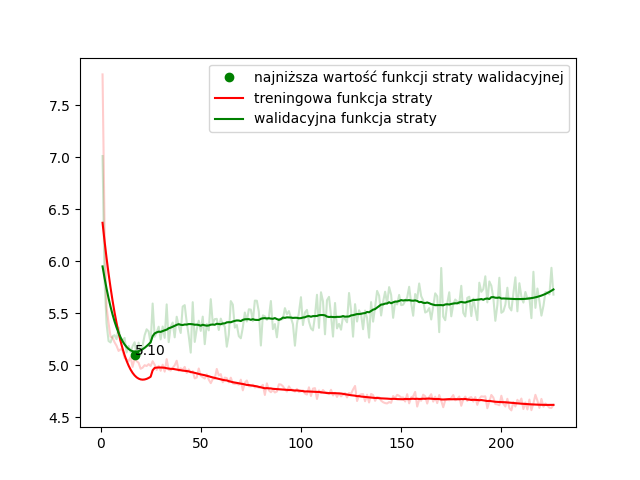
\includegraphics[width=.85\linewidth]{training/alexnet_rnn}
    \caption{Wykres wartości funkcji straty treningowej oraz walidacyjnej dla architektury składającej się z sieci AlexNet i RNN. Opracowanie własne.}
    \label{fig:training-alexnet-rnn}
\end{figure}
\noindent Architektura z wartością funkcji straty na poziomie 5 generowała zdania zawierające jedynie literę „a”, ponieważ jest ona jednym z najczęściej występujących słów w języku angielskim. Wyjątkiem w przypadku wykorzystania sieci RNN jest jej połączenie z transformerem wizyjnym. Dla takiego połączenia metryka BLEU wynosi jedynie 0,01, jednakże wartość CIDEr jest już znacznie wyższa i wynosi 0,13. Wynika to z tego, iż modelowi nie udało się wygenerować pełnych zdań, a jedynie pojedyncze słowa. Przykładowe wyniki zostały przedstawione na rysunku \ref{fig:results-vit-rnn}. Metryka BLEU bierze pod uwagę długość wygenerowanego podpisu, dlatego też w przypadku wygenerowania jedynie pojedynczego słowa, wartość tej metryki jest o wiele niższa w porównaniu do metryki CIDEr.
\begin{figure}[H]
    \centering
    \includegraphics[width=.9\linewidth]{results/vit_rnn}
    \caption{Przykładowe obraz wraz z podpisami wygenerowanymi przez architekturę wykorzystującą transformer wizyjny wraz z siecią RNN. Opracowanie własne.}
    \label{fig:results-vit-rnn}
\end{figure}
\noindent W przypadku tego połączenia funkcja straty walidacyjnej wyniosła wartość 4,5, co można zaobserwować na rysunku \ref{fig:training-vit-rnn}.
\begin{figure}[H]
    \centering
    \includegraphics[width=.9\linewidth]{training/vit_rnn}
    \caption{Wykres wartości funkcji straty treningowej oraz walidacyjnej dla architektury składającej się z transformera wizyjnego i sieci RNN. Opracowanie własne.}
    \label{fig:training-vit-rnn}
\end{figure}
\noindent Jest to stosunkowo lepszy wynik od pozostałych architektur zawierających sieć RNN, biorąc również pod uwagę fakt, iż w przeciwieństwie do pozostałych rozwiązań na wykresie funkcji straty widać dalszy potencjał na malenie jej wartości, a co za tym idzie na nawet lepsze wyniki. Niestety ze względu na ograniczenia czasowe narzucony został limit 500 epok treningowych, które architektura łącząca VIT oraz RNN osiągnęła. Jednocześnie warto zauważyć, że wyuczenie modelu zajęło podobny przedział czasowy, co architektura zawierająca sieć GRU oraz LSTM. W obu tych przypadkach średnia potrzebna na przetworzenie jednej epoki treningowej wyniosła mniej niż 30 sekund, co przy 500 epokach treningowych wynosi około 3 godzin, co jest bardzo zadowalającym czasem. Mimo widocznego potencjału sieci RNN w przypadku połączenia z transformerem wizyjnym nie jest to rozwiązanie, które można uznać za satysfakcjonujące, ponieważ w przypadku wykorzystania sieci RNN w połączeniu z innymi modułami kodującymi, nie udało się osiągnąć zadowalających wyników, a w przypadku wykorzystania transformerów wizyjnych, nie jest to rozwiązanie wydajne ze względu na potrzebę wykorzystania takich samych zasobów komputerowych jak w przypadku wykorzystania sieci GRU lub LSTM. Patrząc na krzywą funkcji straty architektury VIT wraz z siecią GRU widoczne na rysunku \ref{fig:training-vit-gru} można zauważyć jej spłaszczenie w ostatnich epokach treningowych, co nie jest widoczne w przypadku wcześniej omawianego połączenia VIT oraz RNN, jak również w przypadku VIT wraz z klasycznym transformerem, co zostało przedstawione na rysunku \ref{fig:training-vit-transformer}.
\begin{figure}[H]
    \centering
    \begin{subfigure}{.5\textwidth}
        \centering
        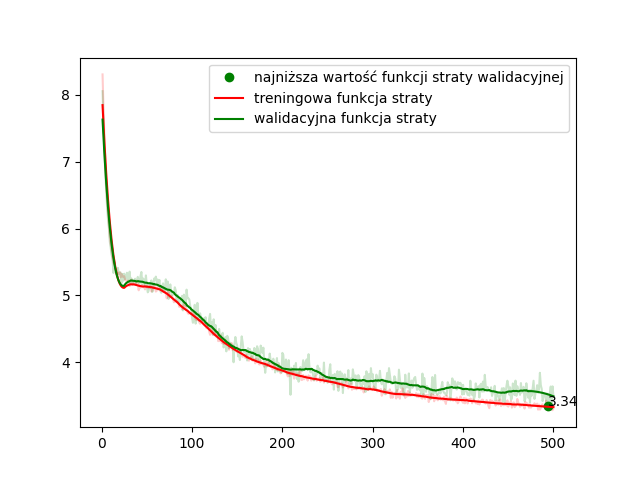
\includegraphics[width=.99\linewidth,trim={1cm 0 1cm 0},clip]{training/vit_gru}
        \caption{GRU}
        \label{fig:training-vit-gru}
    \end{subfigure}%
    \centering
    \begin{subfigure}{.5\textwidth}
        \centering
        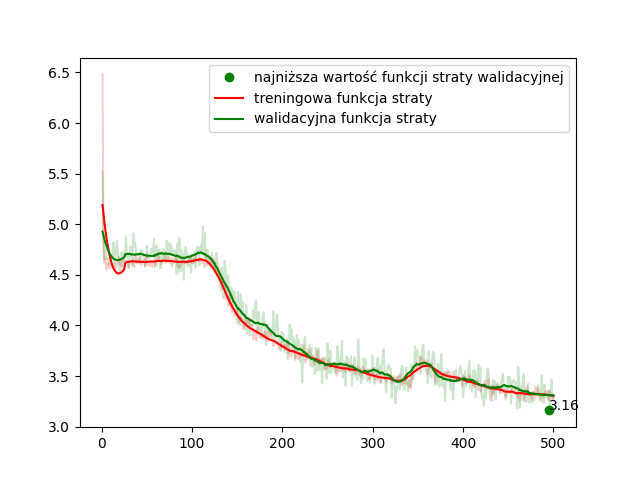
\includegraphics[width=.99\linewidth,trim={1cm 0 1cm 0},clip]{training/vit_transformer_v2}
        \caption{Transformer}
        \label{fig:training-vit-transformer}
    \end{subfigure}%
    \caption{Wykres wartości funkcji straty treningowej oraz walidacyjnej dla architektury składającej się z transformera wizyjnego wraz z różnymi modułami dekodującymi. Opracowanie własne.}
    \label{fig:training-vit-gru-transformer}
\end{figure}
% \begin{figure}[H]
%     \centering
%     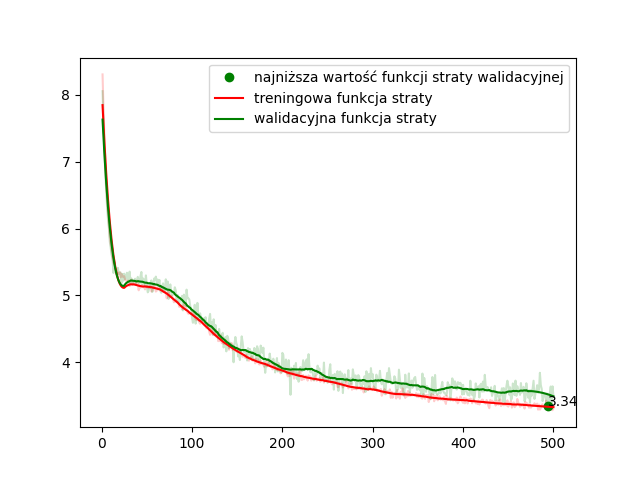
\includegraphics[width=.9\linewidth]{training/vit_gru}
%     \caption{Wykres wartości funkcji straty treningowej oraz walidacyjnej dla architektury składającej się z transformera wizyjnego i sieci GRU. Opracowanie własne.}
%     \label{fig:training-vit-gru}
% \end{figure}
% \begin{figure}[H]
%     \centering
%     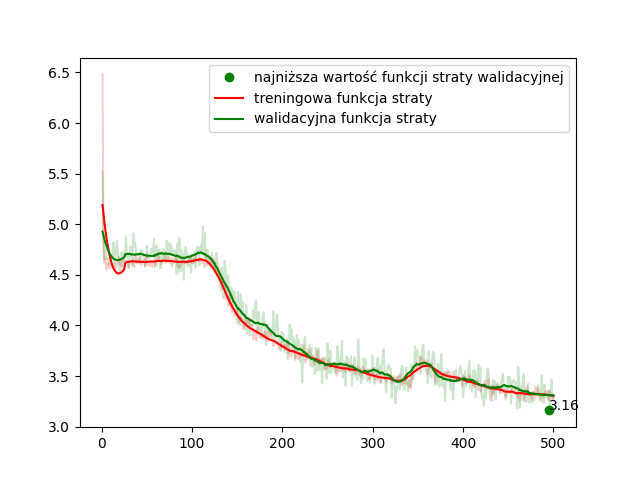
\includegraphics[width=.9\linewidth]{training/vit_transformer_v2}
%     \caption{Wykres wartości funkcji straty treningowej oraz walidacyjnej dla architektury składającej się z transformera wizyjnego i klasycznego. Opracowanie własne.}
%     \label{fig:training-vit-transformer}
% \end{figure}
\noindent Przypadek architektury zawierającej transformer wizyjny i klasyczny jest o wiele bardziej obiecujący niż w przypadku wykorzystania sieci RNN. Wartości funkcji straty są znacznie niższe, widoczna jest dalsza tendencja spadkowa krzywej, a co za tym idzie, możliwe byłoby dalsze poprawianie wyników. Niestety wykorzystywanie klasycznego transformera wiąże się z o wiele większym zapotrzebowaniem zasobów komputerowych. Przetworzenie jednej epoki treningowej architektury VIT i Transformer zajęło średnio 51 sekund, co jest wynikiem prawie dwa razu większym niż w przypadku wykorzystania sieci RNN, GRU lub LSTM. Przykładowe podpisy wygenerowane przez tę architekturę zostały przedstawione na rysunku \ref{fig:results-vit-transformer}.
\begin{figure}[H]
    \centering
    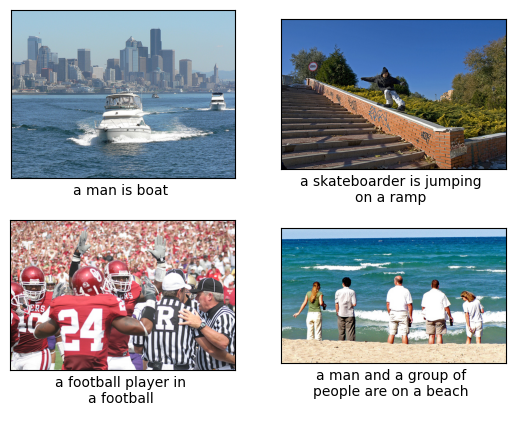
\includegraphics[width=.9\linewidth]{results/vit_transformer}
    \caption{Przykładowe obrazy wraz z podpisami wygenerowanymi przez architekturę wykorzystującą transformer wizyjny wraz z klasycznym transformerem. Opracowanie własne.}
    \label{fig:results-vit-transformer}
\end{figure}
\noindent Można zaobserwować, iż wygenerowane podpisy są o wiele dłuższe niż w porównaniu do architektury VIT i RNN, jednakże brakuje im logicznej spójności. W dużej mierze są one bez sensu, ale zawarte w nich rzeczowniki w większości odnoszą się do faktycznych obiektów znajdujących się na zdjęciach. Jest to dosyć logiczne ze względu na wykorzystanie wstępnie wyuczonych modułów kodujących, które były trenowane na zbiorze danych przeznaczonym do zadań klasyfikacyjnych. Wskazuje to na poprawne rozpoznawanie obiektów znajdujących się na obrazie, jednakże architektura nie potrafi ich połączyć w logiczną całości, za co odpowiedzialny jest moduł dekodujący generujący sekwencję. Mimo wykorzystania zaawansowanego modułu dekodującego, jakim jest transformer, jego danymi wejściowymi cały czas jest pojedynczy wektor reprezentujący obraz. Natomiast podpisy wygenerowane przez sieć GIT, widoczne na rysunku \ref{fig:results-git}, są o wiele bardziej zadowalające, tworzą one zrozumiałe zdania i można zauważyć w nich identyfikacje odpowiednich relacji pomiędzy obiektami znajdującymi się na zdjęciach.
\begin{figure}[H]
    \centering
    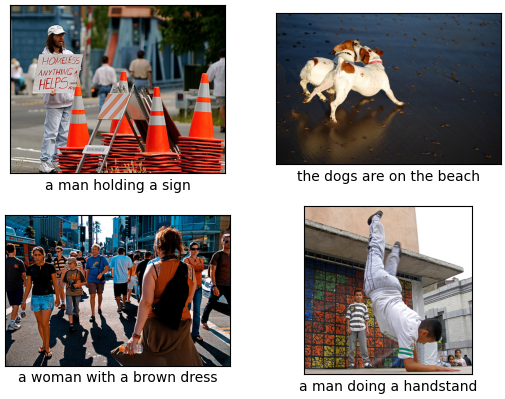
\includegraphics[width=.9\linewidth]{results/git_results}
    \caption{Przykładowe obrazy wraz z podpisami wygenerowanymi przez architekturę GIT. Opracowanie własne.}
    \label{fig:results-git}
\end{figure}
\noindent Tak dobry wynik w porównaniu do pozostałych architektur pokazuje duży wpływ modułu dekodującego na ostateczny rezultat oraz możliwości analizowania obrazu jako całą sekwencję, a nie tylko jako pojedynczy element początkowy. W przypadku tejże sieci warto również przypomnieć, iż w ramach testów wykorzystany został wcześniej wytrenowany model na zbiorze MS COCO, który nie był dostrojony do zbioru Flickr. Niestety tak dobra skuteczność oraz duży potencjał wiążą się z bardzo dużym zapotrzebowaniem na zasoby komputerowe. Wykorzystanie tego rozwiązania zajmuje bardzo dużo czasu i ze względu na ogromną liczbę parametrów nie jest możliwe jego użycie przy pomocy mniejszych kart graficznych, co znacząco wpływa na czas przetwarzania. W przypadku wykorzystania modelu wstępnie wyuczonego takie ograniczenia mogą nie być dużą przeszkodą, ale na pewno korzystając z modelu bez wstępnych wartości parametrów architektury, otrzymanie tak dobrego wyniku może okazać się nieosiągalne ze względu na ograniczenia zasobów komputerowych, czasowych lub budżetowych.

Warto również zwrócić uwagę na wyniki architektury wykorzystującej splotową sieć AlexNet. Rysunek \ref{fig:metrics-transformer} przedstawia wartości metryk wszystkich modułów kodujących w połączeniu z transformerem jako modułem dekodującym. Można na nim zauważyć bardzo dobry wynik w porównaniu do pozostałych architektur.
\begin{figure}[H]
    \centering
    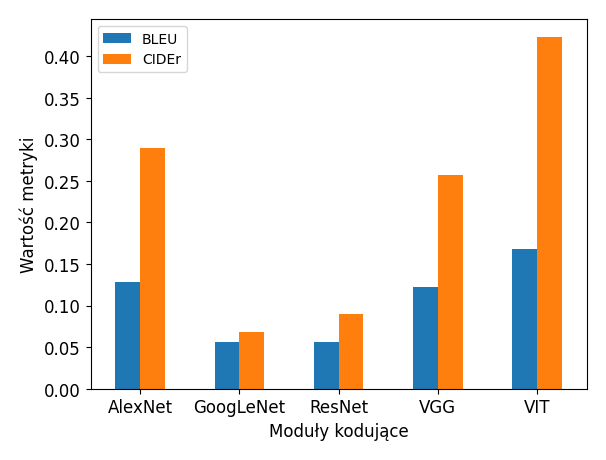
\includegraphics[width=.9\linewidth]{metrics/transformer_metrics}
    \caption{Wartości metryk BLEU oraz CIDEr dla poszczególnych modułów kodujących połączonych z transformerem jako modułem dekodującym. Opracowanie własne.}
    \label{fig:metrics-transformer}
\end{figure}
\noindent Sieć AlexNet ustąpiła jedynie miejsca architekturze GIT oraz kombinacjom modułów wykorzystujących transformer wizyjny. Wynika to z faktu, iż posiadała ona największą ostatnią warstwę w swojej architekturze. Zawierała ona ponad 4 tysiące parametrów -- GoogLeNet, ResNet posiadały ich zdecydowanie mniej, ponieważ odpowiednio: 1024 oraz 2048. Przykładowe podpisy wygenerowane przez architekturę AlexNet wraz z transformerem zostały przedstawione na rysunku \ref{fig:results-alexnet-transformer}. Są one dosyć podobne jakościowo do tych otrzymanych przy pomocy VIT.
\begin{figure}[H]
    \centering
    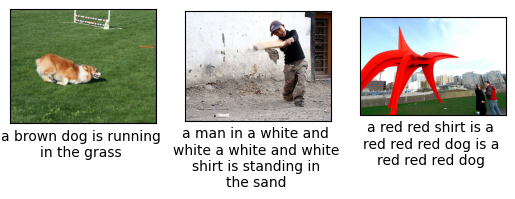
\includegraphics[width=.9\linewidth]{results/alexnet_transformer}
    \caption{Przykładowe obraz wraz z podpisami wygenerowanymi przez architekturę wykorzystującą transformer wizyjny wraz z siecią RNN. Opracowanie własne.}
    \label{fig:results-alexnet-transformer}
\end{figure}
\noindent Zaskakujący jest słabszy wynik architektury VGG, która posiadała taką samą liczbę parametrów jak AlexNet, a mimo wszystko okazała się mniej skuteczna w przypadku obu metryk. Ponownie można zwrócić uwagę na bardzo duży wpływ w analizowaniu obrazu poprzez wykorzystanie transformera wizyjnego, ponieważ pomimo posiadania najmniejszej liczby parametrów -- jedynie 768 -- architektury go wykorzystujące osiągnęły zdecydowanie najlepsze wyniki. Nie można jednocześnie zapomnieć o bardzo dużym wpływie liczby parametrów na czas potrzebny do wyuczenia danych architektur, które można zaobserwować na rysunku \ref{fig:timings-training-decoders-nvidia} dla karty graficznej Nvidia T4.
\begin{figure}[H]
    \centering
    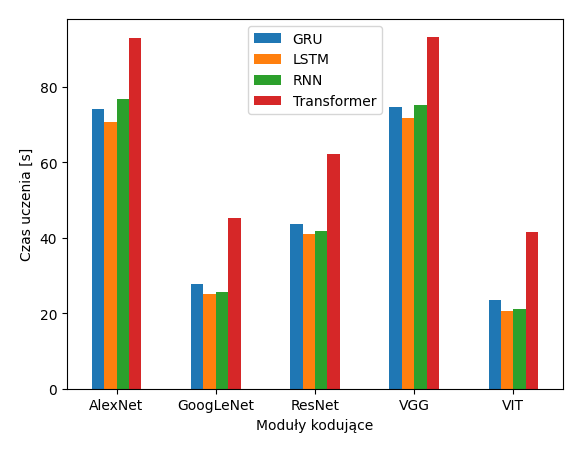
\includegraphics[width=.95\linewidth]{timings/timings_training_decoders_nvidia}
    \caption{Czas przetwarzania jednej epoki treningowej przy użyciu kart graficznej Nvidia T4 dla poszczególnych modułów dekodujących wykorzystujących wstępnie wyuczone moduły kodujące. Opracowanie własne.}
    \label{fig:timings-training-decoders-nvidia}
\end{figure}
\noindent Widoczny jest bezpośredni wpływ liczby parametrów modułów kodujących na czas przetwarzania. Jest to przewidywalnym wynikiem, ponieważ w przypadku większej ilości danych, sieć rekurencyjna musi przetworzyć ich stosunkowo więcej. Interesującym jest fakt, iż nie miało to bezpośredniego przełożenia na lepsze wyniki. Pokazuje to, iż bardzo istotne jest przeanalizowanie obrazu w odpowiedni sposób i najpewniej zwiększenie liczby parametrów w modułach kodujących miałoby w pewnym stopniu wpływ na poprawę skuteczności generowania podpisów, ale porównując różnice w przypadku takich sieci jak GoogLeNet, ResNet, VGG nie są one drastyczne. Warte zweryfikowania na pewno byłoby zwiększenie tejże ilości w przypadku transformera wizyjnego.
\subsection{Skuteczność architektury wykorzystującej zaproponowane połączenie}
Skuteczność rozwiązania wykorzystującego dane pochodzące z pośrednich warstw splotowych została przedstawiona na rysunku \ref{fig:metrics-modified}.
\begin{figure}[H]
    \centering
    \begin{subfigure}{.5\textwidth}
        \centering
        \includegraphics[width=.95\linewidth]{metrics/metrics_modified/BLEU}
        \caption{Wartości metryki BLEU}
        \label{fig:bleu-modified}
    \end{subfigure}%
    \centering
    \begin{subfigure}{.5\textwidth}
        \centering
        \includegraphics[width=.95\linewidth]{metrics/metrics_modified/CIDEr}
        \caption{Wartości metryki CIDEr}
        \label{fig:cider-modified}
    \end{subfigure}%
    \caption{Wartości metryk BLEU oraz CIDEr dla poszczególnych kombinacji modułów kodujących i dekodujących wykorzystujących zaproponowane połączenie. Opracowanie własne}
    \label{fig:metrics-modified}
\end{figure}
\noindent Ponownie można zauważyć, iż sieć RNN nie poradziła sobie z tym zadaniem i nie osiągnęła sensownych rezultatów -- dla każdej architektury splotowej wartość metryk wyniosła zero. W przypadku pozostałych modułów dekodujących otrzymane wyniki są do siebie zbliżone. Wyniki poszczególnych sieci splotowych są na bardzo zbliżonym poziomie, w przeciwieństwie do architektury z klasycznym połączeniem. Taki stan rzeczy wynika z faktu, iż wektor wyjściowy każdego modułu kodującego był takiego samego rozmiaru -- w przypadku architektury klasycznego połączenia wektory te różniły się rozmiarem, co miało bezpośredni wpływ na skuteczność danej architektury. W przypadku wykorzystania danych z warstw pośrednich każdy wektor był długości 4096. Taki rezultat sugeruje, iż bardzo istotne jest zawarcie jak największej ilości danych przekazywanych do modułu dekodującego.

Na podstawie krzywych funkcji straty można zauważyć, iż w przypadku wykorzystania danych z warstw splotowych różnice pomiędzy wartościami zbioru walidacyjnego i treningowego są znacznie większe niż w przypadku klasycznego połączenia modułów, co można zaobserwować na rysunku \ref{fig:training-alexnet-gru-modified}, który przedstawia dane treningowe architektury składającej się z sieci AlexNet oraz GRU.
\begin{figure}[H]
    \centering
    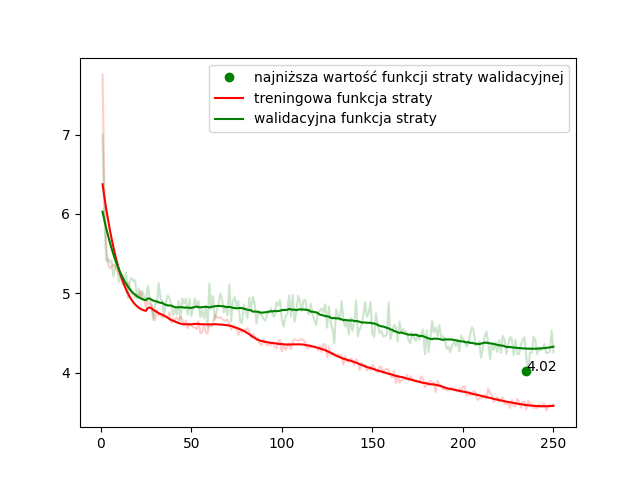
\includegraphics[width=.95\linewidth]{training/alexnet_gru_modified}
    \caption{Wykres wartości funkcji straty treningowej oraz walidacyjnej dla architektury składającej się z sieci AlexNet i GRU. Opracowanie własne.}
    \label{fig:training-alexnet-gru-modified}
\end{figure}
\noindent Mimo iż najlepsza wartość funkcji straty została osiągnięta przy końcu treningu, to już od połowy wartość walidacyjna nie spadała w takim samym tempie, co wartość funkcji straty na zbiorze treningowym. Może to świadczyć o zbyt małej generalizacji danych wejściowych. Można wysunąć wniosek, iż wykorzystywanie danych z warstw splotowych nie jest tak efektywne, ponieważ są to dane zbyt ogólne, niezawierające kluczowych informacji o charakterystyce obrazu.

Podpisy wygenerowane przez większość kombinacji zawierających GRU lub LSTM jako moduł dekodujący wraz z pozostałym modułami kodującymi są bardzo podobne do siebie, co jest przewidywalnym rezultatem na podstawie wartości metryk, jak również krzywych funkcji straty dla tychże rozwiązań. Przykładowe podpisy wygenerowane przez architekturę wykorzystującą AlexNet wraz z LSTM zostały przedstawione na rysunku \ref{fig:results-alexnet-lstm-modified}.
\begin{figure}[H]
    \centering
    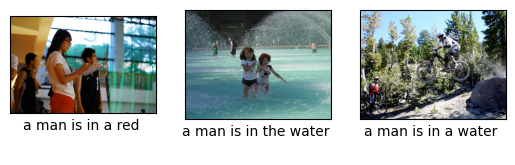
\includegraphics[width=.8\linewidth,trim={0 0.5cm 0 0.25cm},clip]{results/alexnet_lstm_results}
    \caption{Przykładowe obrazki wraz z podpisami wygenerowanymi przez architekturę wykorzystującą sieć VGG i GRU połączone przy pomocy rozwiązania wykorzystującego dane z pośrednich warstw splotowych. Opracowanie własne.}
    \label{fig:results-alexnet-lstm-modified}
\end{figure}
\noindent Można zauważyć, iż wygenerowane podpisy tworzą pełne zdania, jednakże znacząco odbiegają one od kontekstu zawartego na zdjęciach. Pojedyncze wyrazy faktycznie korespondują do obiektów znajdujących się na fotografiach, ale ich połączenie w logiczną całość jest nieodpowiednie. Taki stan rzeczy sugeruje, iż być może moduły kodujące za bardzo skupiają się na wyodrębnianiu informacji dotyczących identyfikacji konkretnych obiektów, a zbyt małe zaawansowanie modułów dekodujących nie pozwala na zbyt zaawansowane zinterpretowanie związków przyczynowo skutkowych znajdujących się na obrazkach.
\subsection{Porównanie z innymi rozwiązaniami}
Najlepszą z architektur łączących bezpośrednio moduły kodujące i dekodujące okazało się połączenie transformera wizyjnego wraz z klasycznym transformerem, które wykorzystywało proste połączenie modułów. W przypadku połączenie uwzględniającego dane z warstw splotowych najlepszym rozwiązaniem okazało się połączeniem sieci ResNet oraz Transformera, jednakże metryki przez nie otrzymane były prawie dwukrotnie mniejsze niż wcześniej wspomniane rozwiązanie. Mimo to wartości metryk otrzymane przy pomocy obu rozwiązań mocno odstają od tych otrzymanych przy pomocy dedykowanych rozwiązań takich jak GIT oraz OFA, co zostało przedstawione w tabeli \ref{tab:comparison}. W przypadku rozwiązania GIT oraz OFA zostały tam umieszczone wyniki podane bezpośrednio przez autorów, jak również te otrzymane przy pomocy udostępnionych wstępnie wyuczonych modeli, które zostały wygenerowane poprzez wykorzystanie tego samego zbioru danych testowych, jak w przypadku pozostałych rozwiązań wykorzystujących połączenie modułu kodującego oraz dekodującego, co pozwoliło na bezpośrednie porównanie tychże rozwiązań, co okazuje się kluczowe ze względu na spore rozbieżności wyników otrzymanych przez autorów oraz w drodze testowania.
\begin{table}[H]
    \centering
    \caption{Porównanie skuteczności rozwiązania wykorzystującego VIT oraz transformera wizyjnego z innymi rozwiązaniami.}
    \label{tab:comparison}
    \begin{tabular}{|l|l|l|l|l|}
        \hline
        \textbf{Rozwiązanie} & \textbf{BLEU} & \textbf{METEOR} & \textbf{CIDEr} & \textbf{SPICE} \\ \hline
        VIT + Transformer    & 0,17          & 0,18            & 0,42           & 0,10           \\ \hline
        GIT (test)           & 0,19          & 0,17            & 0,58           & 0,13           \\ \hline
        GIT (artykuł)        & 0,40          & 0,30            & 1,31           & 0,23           \\ \hline
        OFA (test)           & 0,33          & 0,28            & 1,03           & 0,21           \\ \hline
        OFA  (artykuł)       & 0,43          & 0,32            & 1,45           & 0,25           \\ \hline
    \end{tabular}
\end{table}
\noindent Wartości metryk otrzymane dla architektury GIT w przypadku BLEU oraz METEOR są nieznacznie wyższe od rozwiązania VIT + Transformer. W przypadku metryk CIDEr i SPICE różnice są bardziej zauważalne, co może świadczyć o lepszej zdolności GIT do zachowania sensu i semantyki w generowanych podpisach. Jednakże porównując wyniki GIT z tymi podanymi bezpośrednio przez autorów architektury, zauważalne są znaczne różnice. Wartości wszystkich metryk dla testowanego wariantu są prawie dwukrotnie mniejsze niż te, które podali autorzy. Takie rozbieżności mogą wskazywać na słabą zdolność architektury do generalizacji na różne zbiory danych, ponieważ wyniki przez nich podane zostały otrzymane przy pomocy zbioru MS COCO, natomiast zbiorem wykorzystanym do otrzymania testowych wyników był Flickr8k. Na tak duże różnice również mogły mieć specyficzne warunki testowe lub wadliwość modelu przekazanego przez autorów. W przypadku architektury OFA, różnice między wartościami otrzymanymi w badaniach a tymi zawartymi w artykule są niewielkie. Wartości wszystkich metryk podane przez autorów są większe o kilka setnych, co sugeruje, że OFA utrzymuje stabilność wyników i skuteczność w różnych kontekstach. Może to wskazywać na lepszą generalizację i niezawodność architektury OFA w porównaniu do GIT, która również osiągnęła największe wartości w przypadku wszystkich podanych metryk. Jest to przewidywalnym rezultatem, ponieważ OFA została stworzona z myślą o generalizacji i zdolności rozwiązywania wielu różnych zadań z dziedziny przetwarzania obrazu oraz generowania tekstu.

Patrząc na to, iż tak duża przepaść dzieli rozwiązania wykorzystujące proste połączenie modułów kodującego i dekodującego do dedykowanych rozwiązań, można wysunąć wniosek, iż kluczowym jest odpowiednie wykorzystanie danych wejściowych. Dedykowane rozwiązania interpretują obraz jako sekwencję, co pozwala na bardziej złożoną analizę obrazu, a co za tym idzie na bardziej złożone generowanie podpisów. W przypadku wykorzystania klasycznego połączenia modułów kodującego i dekodującego obraz jest interpretowany jako pojedynczy element, co ogranicza możliwości analizy obrazu, ale było konieczne ze względu na rodzaj danych wejściowych sieci rekurencyjnych. W przypadku wykorzystania transformera, mimo jego możliwości przetwarzania sekwencji oraz wykorzystywania modułu atencji, w celu utrzymania modularnej architektury, danymi wejściowymi również był pojedynczy element sekwencji.
% TODO dopisać ze trzy zdania